% Paired assistance differences with 95 percent intervals, per sample (email and production).
\begin{figure}[htbp]
\centering
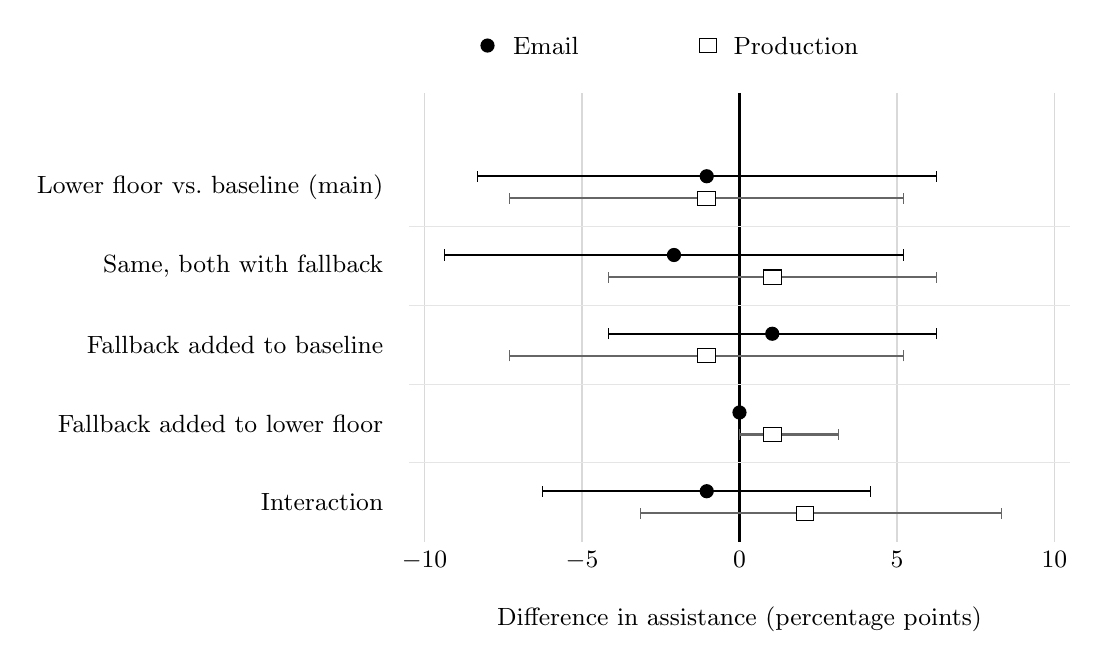
\begin{tikzpicture}[x=0.4cm,y=1cm,font=\small]
  \foreach \p in {-10,-5,0,5,10} {
    \draw[black!15] (\p,0.7) -- (\p,-5.0);
    \node[below] at (\p,-5.0) {$\p$};
  }
  \draw[thick] (0,0.7) -- (0,-5.0);
  \node[below] at (0,-5.7) {Difference in assistance (percentage points)};
  \node[left] at (-11,-0.5) {Lower floor vs.\ baseline (main)};
  \node[left] at (-11,-1.5) {Same, both with fallback};
  \node[left] at (-11,-2.5) {Fallback added to baseline};
  \node[left] at (-11,-3.5) {Fallback added to lower floor};
  \node[left] at (-11,-4.5) {Interaction};
  \foreach \y in {-1,-2,-3,-4} {
    \draw[black!10] (-10.5,\y) -- (10.5,\y);
  }
  % email: filled circle, upper offset
  \foreach \y/\m/\lo/\hi in {-0.36/-1.04/-8.33/6.25, -1.36/-2.08/-9.38/5.21, -2.36/1.04/-4.17/6.25, -3.36/0.00/0.00/0.00, -4.36/-1.04/-6.25/4.17} {
    \draw[thick] (\lo,\y) -- (\hi,\y);
    \draw (\lo,\y-0.07) -- (\lo,\y+0.07);
    \draw (\hi,\y-0.07) -- (\hi,\y+0.07);
    \fill (\m,\y) circle (0.9mm);
  }
  % production: open square, lower offset
  \foreach \y/\m/\lo/\hi in {-0.64/-1.04/-7.29/5.21, -1.64/1.04/-4.17/6.25, -2.64/-1.04/-7.29/5.21, -3.64/1.04/0.00/3.13, -4.64/2.08/-3.13/8.33} {
    \draw[thick,black!60] (\lo,\y) -- (\hi,\y);
    \draw[black!60] (\lo,\y-0.07) -- (\lo,\y+0.07);
    \draw[black!60] (\hi,\y-0.07) -- (\hi,\y+0.07);
    \draw[fill=white] (\m-0.28,\y-0.09) rectangle (\m+0.28,\y+0.09);
  }
  \fill (-8,1.3) circle (0.9mm);
  \node[right] at (-7.5,1.3) {Email};
  \draw[fill=white] (-1.28,1.21) rectangle (-0.72,1.39);
  \node[right] at (-0.5,1.3) {Production};
\end{tikzpicture}
\caption[Paired assistance differences between retrieval policies, with 95\% question-group bootstrap intervals, for the email and production samples]{Paired assistance differences between retrieval policies, with 95\% question-group bootstrap intervals, for the email and production samples. All intervals include zero. The email interval for adding the fallback to the lower floor is a single point at zero, because with the lower floor both fallback settings select identical contexts for all 96 questions. The values are in Table~\ref{tab:luna-effects}.}
\label{fig:policy-effects}
\end{figure}
